\documentclass[conference]{IEEEtran}
\IEEEoverridecommandlockouts
% The preceding line is only needed to identify funding in the first footnote. If that is unneeded, please comment it out.
\usepackage{cite}
\usepackage{amsmath,amssymb,amsfonts}
\usepackage{algorithmic}
\usepackage{graphicx}
\usepackage{textcomp}
\usepackage{xcolor}
\usepackage{subfig}
\usepackage{float}

\def\BibTeX{{\rm B\kern-.05em{\sc i\kern-.025em b}\kern-.08em
    T\kern-.1667em\lower.7ex\hbox{E}\kern-.125emX}}
\begin{document}

\title{MO443 - Assignment II}

\author{210404 -- Guilherme Vieira Leite}

\maketitle

\section{Introduction}
Segmentation is a vast field of research in computer vision, for its especially known applications in various industries, either to help count objects or highlighting regions of interest. In this work, we explore a few segmentations obtained by thresholds alone. More specifically we explore the strengths and weaknesses of the global threshold and a few local thresholds. This work is organized in the following manner: Section~\ref{sec:method} explains our methods, Section~\ref{sec:result} shows the obtained results, their parameters, and their histograms, and Section~\ref{sec:conclusion} reflects on our results and discuss a few next steps to explore in threshold segmentation.
\section{Methods}
\label{sec:method}
In this section, we explain each of the methods used to perform the segmentation. Our methods were split between global and local ones and their results are illustrated in Section~\ref{sec:result}.\par
Our first and simplest method was the global threshold, in which value $T$ was chosen and every pixel was segmented according to $T$. This method has a predetermined belief that the foreground and background of the image are well distributed in the histogram and can be split by a single $T$ value.\par
In contrast to the global threshold, and to account for more life scenarios, we also explored local thresholds, in which each pixel has a different $T$ value according to the local neighborhood, of $n$ size, and the chosen method. The chosen methods and their formulas are the following, with $z(x, y)$ being the region around $pixel(x, y)$: Bernsen Eq.~\ref{eq:bernsen}, Niblack Eq.~\ref{eq:niblack},Sauvola Eq.~\ref{eq:sauvola}, Phansalskar Eq.~\ref{eq:phansalskar}, Contrast Eq.~\ref{eq:contrast}, Mean Eq.~\ref{eq:mean}, and Median Eq.~\ref{eq:median}.
\begin{equation}
\label{eq:bernsen}
    T(x, y) = \frac{z_{min}(x, y) + z_{max}(x, y)}{2}
\end{equation}
\begin{equation}
\label{eq:niblack}
    T(x, y) = \mu(x, y) + k \sigma(x, y)
\end{equation}
\begin{equation}
\label{eq:sauvola}
    T(x, y) = \mu(x, y) \left[ 1 + k \left(\frac{\sigma(x, y)}{r} - 1\right)\right]
\end{equation}
\begin{equation}
\label{eq:phansalskar}
    T(x, y) = \mu(x, y) \left[ 1 + p e^{-q\mu(x, y)} + k \left( \frac{\sigma(x, y)}{r} - 1 \right) \right]
\end{equation}
\begin{equation}
\label{eq:contrast}
    T(x, y) =
    \begin{cases}
    0,& \texit{if} (x, y)\ closer\ to\ max(z(x, y))\\
    255,& \texit{if} (x, y)\ closer\ to\ min(z(x, y))
    \end{cases}
\end{equation}
\begin{equation}
\label{eq:mean}
    T(x, y) = \mu(z(x, y))
\end{equation}
\begin{equation}
\label{eq:median}
    T(x, y) = median(z(x, y))
\end{equation}
\section{Results}
\label{sec:result}
In this section, we present the obtained results upon implementing the methods from Section~\ref{sec:method}. Firstly we show the results of the global threshold followed by the many variations of local thresholds and their histograms. Our input images are shown in Figure~\ref{fig:input}.
\begin{figure}[htbp]
\centering
\subfloat[Baboon]{
	{
		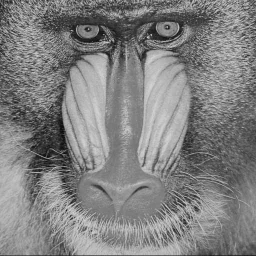
\includegraphics[scale=0.35]{figures/input/baboon}
	}
}
\subfloat[Fiducial]{
	{
		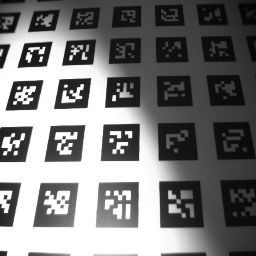
\includegraphics[scale=0.35]{figures/input/fiducial}
	}
}
\quad
\subfloat[Monarch]{
	{
		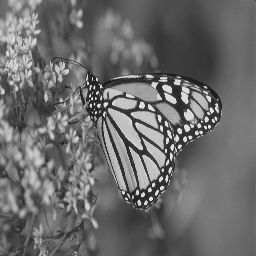
\includegraphics[scale=0.35]{figures/input/monarch}
	}
}
\subfloat[Peppers]{
	{
		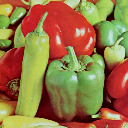
\includegraphics[scale=0.35]{figures/input/peppers}
	}
}
\quad
\subfloat[Retina]{
	{
		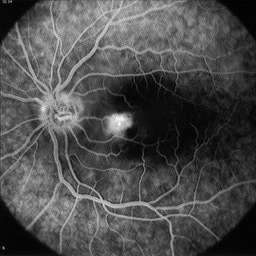
\includegraphics[scale=0.35]{figures/input/retina}
	}
}
\subfloat[Sonnet]{
	{
		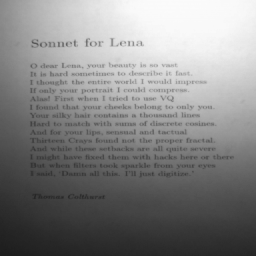
\includegraphics[scale=0.35]{figures/input/sonnet}
	}
}
\caption{A sample of the images used in the experiments.}
\label{fig:input}
\end{figure}
\subsection{Global}
To explore the effects of a global threshold in an image we explored three distinct $T$ values, $T = 50$, $T = 128$, and $T = 200$, shown in Figure~\ref{fig:global_fiducial}. These values were chosen arbitrarily in a manner to explore global threshold's features.
\begin{figure}[htbp]
	\centering
	\subfloat[$T = 50$]{
		{
			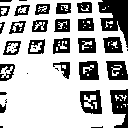
\includegraphics[scale=0.7]{figures/global/global_50_fiducial.png}
		}
		\label{fig:global_50_fiducial}
	}
	\subfloat[$T = 128$]{
		{
			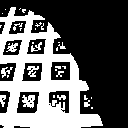
\includegraphics[scale=0.7]{figures/global/global_128_fiducial.png}
		}
		\label{fig:global_128_fiducial}
	}\quad
	\subfloat[$T = 200$]{
		{
			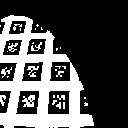
\includegraphics[scale=0.7]{figures/global/global_200_fiducial.png}
		}
		\label{fig:global_200_fiducial}
	}
	\caption{Different $T$s on Fiducial image.}
	\label{fig:global_fiducial}
\end{figure}
In Figure~\ref{fig:global_fiducial} it is possible to notice that a single $T$ value is not enough to distinguish between foreground and background. Figure~\ref{fig:global_50_fiducial} shows a large portion of the foreground, but there is a white spot occluding some of it, this white spot can be seen with different values of $T$, but again it will occlude other parts of the foreground. In general, we obtained a bad performance from lower and higher values of $T$.\par
In Figure~\ref{fig:low_t} it is possible to notice how few features survive the thresholding with a low $T$ value, the worst case being Figure~\ref{fig:low_t_wedge}, which is completely white.
\begin{figure}[htbp]
	\centering
	\subfloat[Baboon]{
		{
			
\includegraphics[scale=0.7]{figures/global/global_50_baboon.png}
		}
		\label{fig:low_t_baboon}
	}
	\subfloat[Monarch]{
		{
			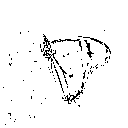
\includegraphics[scale=0.7]{figures/global/global_50_monarch.png}
		}
		\label{fig:low_t_monarch}
	}\quad
	\subfloat[Retina]{
		{
			
\includegraphics[scale=0.7]{figures/global/global_50_retina.png}
		}
		\label{fig:low_t_retina}
	}
	\subfloat[Wedge]{
		{
			
\includegraphics[scale=0.7]{figures/global/global_50_wedge.png}
		}
		\label{fig:low_t_wedge}
	}
	\caption{Low global $T$ on different images.}
	\label{fig:low_t}
\end{figure}
Figure~\ref{fig:high_t} shows the same effect happening with a high $T$ values. We assume this happened because of a somewhat \textit{good} histogram distribution, with dark and light parts in the same image, favoring a more median threshold.
\begin{figure}[htbp]
	\centering
	\subfloat[Baboon]{
		{
			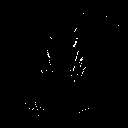
\includegraphics[scale=0.7]{figures/global/global_200_baboon.png}
		}
		\label{fig:high_t_baboon}
	}
	\subfloat[Monarch]{
		{
			
\includegraphics[scale=0.7]{figures/global/global_200_monarch.png}
		}
		\label{fig:high_t_monarch}
	}\quad
	\subfloat[Retina]{
		{
			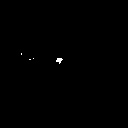
\includegraphics[scale=0.7]{figures/global/global_200_retina.png}
		}
		\label{fig:high_t_retina}
	}
	\subfloat[Wedge]{
		{
			
\includegraphics[scale=0.7]{figures/global/global_200_wedge.png}
		}
		\label{fig:high_t_wedge}
	}
	\caption{High global $T$ on different images.}
	\label{fig:high_t}
\end{figure}
The threshold of $T = 128$ was responsible for the best results in our experiments, seen in Figure~\ref{fig:median_t}. In special the Baboon and Monarch in Figures~\ref{fig:median_t_baboon} and~\ref{fig:median_t_monarch}.
\begin{figure}[htbp]
	\centering
	\subfloat[Baboon]{
		{
			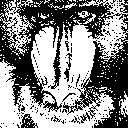
\includegraphics[scale=0.7]{figures/global/global_128_baboon.png}
		}
		\label{fig:median_t_baboon}
	}
	\subfloat[Monarch]{
		{
			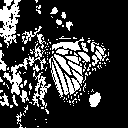
\includegraphics[scale=0.7]{figures/global/global_128_monarch.png}
		}
		\label{fig:median_t_monarch}
	}\quad
	\subfloat[Retina]{
		{
			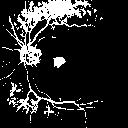
\includegraphics[scale=0.7]{figures/global/global_128_retina.png}
		}
		\label{fig:median_t_retina}
	}
	\subfloat[Wedge]{
		{
			
\includegraphics[scale=0.7]{figures/global/global_128_wedge.png}
		}
		\label{fig:median_t_wedge}
	}
	\caption{Global $T = 128$ on different images.}
	\label{fig:median_t}
\end{figure}
\subsection{Local}
We also explored and compared the effects of the seven local thresholds presented in Section~\ref{sec:method}. Their histograms are shown separately in Subsection~\ref{sec:hist}.
\paragraph*{Bernsen} Figure~\ref{fig:bernsen_n} shows the different aspects of the area considered upon determining the threshold for each pixel. A larger area cleared a lot of the background noise but also corroded some of the borders on the right side of Figure~\ref{fig:bernsen_11_wedge}.
\begin{figure}[htbp]
	\centering
	\subfloat[3x3]{
		{
			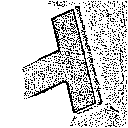
\includegraphics[scale=0.7]{figures/local/bernsen/local_ber_3_wedge.png}
		}
		\label{fig:bernsen_3_wedge}
	}
	\subfloat[7x7]{
		{
			
\includegraphics[scale=0.7]{figures/local/bernsen/local_ber_7_wedge.png}
		}
		\label{fig:bernsen_7_wedge}
	}\quad
	\subfloat[11x11]{
		{
			
\includegraphics[scale=0.7]{figures/local/bernsen/local_ber_11_wedge.png}
		}
		\label{fig:bernsen_11_wedge}
	}
	\caption{Bernsen with different neighbourhoods $n$ on Wedge image.}
	\label{fig:bernsen_n}
\end{figure}
It is also interesting to compare the Bernsen local threshold with the global one. Figure~\ref{fig:global_vs_local} shows the Wedge image, previously badly segmented via global threshold, and now presents some distinguishable features.
\begin{figure}[htbp]
	\centering
	\subfloat[Global]{
		{
			
\includegraphics[scale=0.7]{figures/global/global_128_wedge.png}
		}
		\label{fig:global_vs_local_global}
	}
	\subfloat[Local]{
		{
			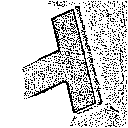
\includegraphics[scale=0.7]{figures/local/bernsen/local_ber_3_wedge.png}
		}
		\label{fig:global_vs_local_local}
	}
	\caption{Global vs Local threshold on Wedge image.}
	\label{fig:global_vs_local}
\end{figure}
\paragraph*{The Niblack} method varies with the neighborhood area $n$, and by the same $k$ factor as Bernsen. Figure~\ref{fig:niblack_n} shows how the $n$ area affects the segmentation, although the three $n$ values segmented the optical nerve, only $n = 11$ showed a clear segmentation of the spot in the center of the image. Upon varying the $k$ value in Figure~\ref{fig:niblack_k} it is noticeable how $k$ affects the border by completely vanishing the image, if the value gets too high, generating a better or worse segmentation.
\begin{figure}[htbp]
	\centering
	\subfloat[3x3]{
		{
			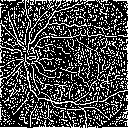
\includegraphics[scale=0.7]{figures/local/niblack/local_nib_3_retina.png}
		}
		\label{fig:niblack_3_retina}
	}
	\subfloat[7x7]{
		{
			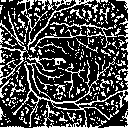
\includegraphics[scale=0.7]{figures/local/niblack/local_nib_7_retina.png}
		}
		\label{fig:niblack_7_retina}
	}\quad
	\subfloat[11x11]{
		{
			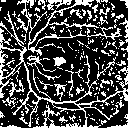
\includegraphics[scale=0.7]{figures/local/niblack/local_nib_11_retina.png}
		}
		\label{fig:niblack_11_retina}
	}
	\caption{Niblack with different neighbourhoods $n$ on Retina image.}
	\label{fig:niblack_n}
\end{figure}
\begin{figure}[htbp]
	\centering
	\subfloat[$k = 0.5$]{
		{
			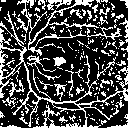
\includegraphics[scale=0.7]{figures/local/niblack/local_nib_11_retina.png}
		}
		\label{fig:niblack_k_0_5_retina}
	}
	\subfloat[$k = 1.0$]{
		{
			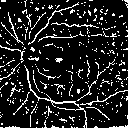
\includegraphics[scale=0.7]{figures/local/niblack/local_nib_11_retina_1_0.png}
		}
		\label{fig:niblack_k_1_0_retina}
	}\quad
	\subfloat[$k = 5.0$]{
		{
			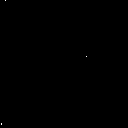
\includegraphics[scale=0.7]{figures/local/niblack/local_nib_11_retina_5_0.png}
		}
		\label{fig:niblack_k_5_0_retina}
	}
	\caption{Niblack with different $k$s on Retina image.}
	\label{fig:niblack_k}
\end{figure}
\paragraph*{The Sauvola and Pietaksinen} methods vary with three parameters, its neighborhood area ($n$), the same border factor from Niblack ($k$), and the maximum standard deviation of the image ($r$). In our experiment, we varied the values of $n$ and $k$ but kept $r = 128$ since all images only varied from 0 to 255 shades of gray.
\begin{figure}[htbp]
	\centering
	\subfloat[3x3]{
		{
			
\includegraphics[scale=0.7]{figures/local/sauvola/local_sau_3_monarch.png}
		}
		\label{fig:sauvola_3_monarch}
	}
	\subfloat[7x7]{
		{
			
\includegraphics[scale=0.7]{figures/local/sauvola/local_sau_7_monarch.png}
		}
		\label{fig:sauvola_7_monarch}
	}\quad
	\subfloat[11x11]{
		{
			
\includegraphics[scale=0.7]{figures/local/sauvola/local_sau_11_monarch.png}
		}
		\label{fig:sauvola_11_monarch}
	}
	\caption{Sauvola with different $n$s on Monarch image.}
	\label{fig:sauvola_n}
\end{figure}
Figure~\ref{fig:sauvola_n} shows the segmentation while varying $n$, in which the best result obtained was using $n = 11$. In Figure~\ref{fig:sauvola_k} we varied $k$ values, and although the recommended value for $k$ is of 0.5, the best segmentation was obtained with $k = 1.0$, seen in Figure~\ref{fig:sauvola_k_1.0_monarch}.
\begin{figure}[htbp]
	\centering
	\subfloat[$k = 0.5$]{
		{
			
\includegraphics[scale=0.7]{figures/local/sauvola/local_sau_11_monarch.png}
		}
		\label{fig:sauvola_k_0.5_monarch}
	}
	\subfloat[$k = 1.0$]{
		{
			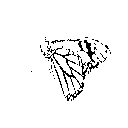
\includegraphics[scale=0.7]{figures/local/sauvola/local_sau_11_monarch_1_0.png}
		}
		\label{fig:sauvola_k_1.0_monarch}
	}\quad
	\subfloat[$k = 5.0$]{
		{
			
\includegraphics[scale=0.7]{figures/local/sauvola/local_sau_11_monarch_5_0.png}
		}
		\label{fig:sauvola_k_5.0_monarch}
	}
	\caption{Sauvola with different $k$s on Monarch image.}
	\label{fig:sauvola_k}
\end{figure}
\paragraph*{The Phansalskar, More and Sabale} method has four parameters, the neighborhood area ($n$), $k$ inherited from the previous methods, and $r$ with a different meaning, and added two new parameters: $p$ and $q$. We faced an error with this method in which the images were only outputting as white images, we tried to normalize the input pixels between 0 and 1, but it did not fix the error in Figure~\ref{fig:phansalskar_n}, which shows our results with varying $n$ and freezing the other parameters to their recommended value: $k = 0.25$, $r = 0.5$, $p = 2$, and $q = 10$.
\begin{figure}[htbp]
	\centering
	\subfloat[3x3]{
		{
			
\includegraphics[scale=0.7]{figures/local/phansalskar/local_pha_3_sonnet.png}
		}
		\label{fig:phansalskar_3}
	}
	\subfloat[7x7]{
		{
			
\includegraphics[scale=0.7]{figures/local/phansalskar/local_pha_7_sonnet.png}
		}
		\label{fig:phansalskar_7}
	}\quad
	\subfloat[11x11]{
		{
			
\includegraphics[scale=0.7]{figures/local/phansalskar/local_pha_11_sonnet.png}
		}
		\label{fig:phansalskar_11}
	}
	\caption{Phansalskar with different $k$s on Sonnet image.}
	\label{fig:phansalskar_n}
\end{figure}
\paragraph*{Contrast} This method varies only by the size of the neighborhood $n$ area. The majority of the contrast results did not produce distinguishable images, as in Figure~\ref{fig:contrast_bad_peppers} with no clear features of the objects. In one instance this method produced a better result on image Sonnet, seen in Figure~\ref{fig:contrast_sonnet}, but still only for small neighborhood areas.
\begin{figure}[htbp]
	\centering
	\subfloat[3x3]{
		{
			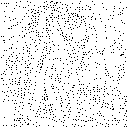
\includegraphics[scale=0.7]{figures/local/contrast/local_con_3_peppers.png}
		}
		\label{fig:contrast_bad_3_peppers}
	}
	\subfloat[7x7]{
		{
			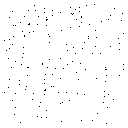
\includegraphics[scale=0.7]{figures/local/contrast/local_con_7_peppers.png}
		}
		\label{fig:contrast_bad_7_peppers}
	}\quad
	\subfloat[11x11]{
		{
			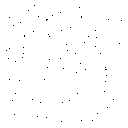
\includegraphics[scale=0.7]{figures/local/contrast/local_con_11_peppers.png}
		}
		\label{fig:contrast_bad_11_peppers}
	}
	\caption{Bad contrast with different neighbourhoods $n$ on Peppers image.}
	\label{fig:contrast_bad_peppers}
\end{figure}
\begin{figure}[htbp]
	\centering
	\subfloat[3x3]{
		{
			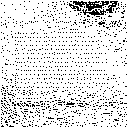
\includegraphics[scale=0.7]{figures/local/contrast/local_con_3_sonnet.png}
		}
		\label{fig:contrast_3_sonnet}
	}
	\subfloat[7x7]{
		{
			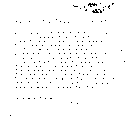
\includegraphics[scale=0.7]{figures/local/contrast/local_con_7_sonnet.png}
		}
		\label{fig:contrast_7_sonnet}
	}\quad
	\subfloat[11x11]{
		{
			
\includegraphics[scale=0.7]{figures/local/contrast/local_con_11_sonnet.png}
		}
		\label{fig:contrast_11_sonnet}
	}
	\caption{Contrast with different neighbourhoods $n$ on Sonnet image.}
	\label{fig:contrast_sonnet}
\end{figure}
\paragraph*{Mean} This method varies only by the size of the neighborhood $n$ area. In Figure~\ref{fig:mean_baboon} it is possible to notice some features of the baboon throughout the different $n$ values, with the smaller windows producing the worst result. Another interesting fact to notice is the noise generated at the borders of the image, it is caused by the padding done via adding $0$s to the image and influencing in the mean calculation.
\begin{figure}[htbp]
	\centering
	\subfloat[3x3]{
		{
			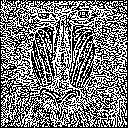
\includegraphics[scale=0.7]{figures/local/mean/local_mea_3_baboon.png}
		}
		\label{fig:mean_3_baboon}
	}
	\subfloat[7x7]{
		{
			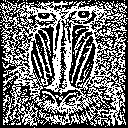
\includegraphics[scale=0.7]{figures/local/mean/local_mea_7_baboon.png}
		}
		\label{fig:mean_7_baboon}
	}\quad
	\subfloat[11x11]{
		{
			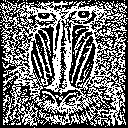
\includegraphics[scale=0.7]{figures/local/mean/local_mea_7_baboon.png}
		}
		\label{fig:mean_11_baboon}
	}
	\caption{Mean with different neighbourhoods $n$ on Baboon image.}
	\label{fig:mean_baboon}
\end{figure}
\paragraph*{Median} This method varies only by the size of the neighborhood $n$ area. Figure~\ref{fig:median_monarch} shows the benefits of a larger area, with more distinguishable features, but still an overall cluttered image.
\begin{figure}[htbp]
	\centering
	\subfloat[3x3]{
		{
			\includegraphics[scale=0.7]{figures/local/median/local_med_3_monarch.png}
		}
		\label{fig:median_3_monarch}
	}
	\subfloat[7x7]{
		{
			\includegraphics[scale=0.7]{figures/local/median/local_med_7_monarch.png}
		}
		\label{fig:median_7_monarch}
	}\quad
	\subfloat[11x11]{
		{
			\includegraphics[scale=0.7]{figures/local/median/local_med_11_monarch.png}
		}
		\label{fig:median_11_monarch}
	}
	\caption{Median with different neighbourhoods $n$ on Monarch image.}
	\label{fig:median_monarch}
\end{figure}
\subsection{Histograms}
\label{sec:hist}
We generated the histograms in Figure~\ref{fig:hist} for each of method reported above on image Monarch, with $n = 3$ and $k = 0.5$.
\section{Conclusion}
\label{sec:conclusion}
In this work, we explored and compared some aspects of global and local thresholding. We went through some well known local methods: (i) Bernsen, (ii) Niblack, (iii) Sauvola, (iv) Phansalskar, (v) Contrast, (vi) Mean, and (vii) Median; and compared some variations of their parameters. Overall the local thresholds were better than the global ones, but they all required some grid search for each application, for instance, the Phansalskar was proposed to be used in biological cells segmentation, and so their recommended parameters are specifically for that use case. Regarding computing time both approaches were fast to execute on a CPU, although, global was faster the difference was minimal. Some few details could be explored in future works such as an extensive grid search for the parameters, and the use of wrap-around padding to avoid dark borders.
\begin{figure*}[htbp]
	\centering
	\subfloat[Bernsen]{
		{
			\includegraphics[scale=0.35]{figures/hist/local_hist_ber_3_monarch.png}
		}
		\label{fig:hist_ber}
	}
	\subfloat[Niblack]{
		{
			\includegraphics[scale=0.35]{figures/hist/local_hist_nib_3_monarch.png}
		}
		\label{fig:hist_nib}
	}\quad
	\subfloat[Sauvola]{
		{
			\includegraphics[scale=0.35]{figures/hist/local_hist_sau_3_monarch.png}
		}
		\label{fig:hist_sau}
	}
	\subfloat[Phansalskar]{
		{
			\includegraphics[scale=0.35]{figures/hist/local_hist_pha_3_monarch.png}
		}
		\label{fig:hist_sau}
	}\quad
	\subfloat[Contrast]{
		{
			\includegraphics[scale=0.35]{figures/hist/local_hist_con_3_monarch.png}
		}
		\label{fig:hist_con}
	}
	\subfloat[Mean]{
		{
			\includegraphics[scale=0.35]{figures/hist/local_hist_mea_3_monarch.png}
		}
		\label{fig:hist_mea}
	}\quad
	\subfloat[Median]{
		{
			\includegraphics[scale=0.35]{figures/hist/local_hist_med_3_monarch.png}
		}
		\label{fig:hist_med}
	}
	\caption{Histogram for $n = 3$ on all images.}
	\label{fig:hist}
\end{figure*}
\end{document}